% Options for packages loaded elsewhere
\PassOptionsToPackage{unicode}{hyperref}
\PassOptionsToPackage{hyphens}{url}
%
\documentclass[
  12pt,
]{article}
\usepackage{lmodern}
\usepackage{amssymb,amsmath}
\usepackage{ifxetex,ifluatex}
\ifnum 0\ifxetex 1\fi\ifluatex 1\fi=0 % if pdftex
  \usepackage[T1]{fontenc}
  \usepackage[utf8]{inputenc}
  \usepackage{textcomp} % provide euro and other symbols
\else % if luatex or xetex
  \usepackage{unicode-math}
  \defaultfontfeatures{Scale=MatchLowercase}
  \defaultfontfeatures[\rmfamily]{Ligatures=TeX,Scale=1}
\fi
% Use upquote if available, for straight quotes in verbatim environments
\IfFileExists{upquote.sty}{\usepackage{upquote}}{}
\IfFileExists{microtype.sty}{% use microtype if available
  \usepackage[]{microtype}
  \UseMicrotypeSet[protrusion]{basicmath} % disable protrusion for tt fonts
}{}
\makeatletter
\@ifundefined{KOMAClassName}{% if non-KOMA class
  \IfFileExists{parskip.sty}{%
    \usepackage{parskip}
  }{% else
    \setlength{\parindent}{0pt}
    \setlength{\parskip}{6pt plus 2pt minus 1pt}}
}{% if KOMA class
  \KOMAoptions{parskip=half}}
\makeatother
\usepackage{xcolor}
\IfFileExists{xurl.sty}{\usepackage{xurl}}{} % add URL line breaks if available
\IfFileExists{bookmark.sty}{\usepackage{bookmark}}{\usepackage{hyperref}}
\hypersetup{
  hidelinks,
  pdfcreator={LaTeX via pandoc}}
\urlstyle{same} % disable monospaced font for URLs
\usepackage[margin=1in]{geometry}
\usepackage{longtable,booktabs}
% Correct order of tables after \paragraph or \subparagraph
\usepackage{etoolbox}
\makeatletter
\patchcmd\longtable{\par}{\if@noskipsec\mbox{}\fi\par}{}{}
\makeatother
% Allow footnotes in longtable head/foot
\IfFileExists{footnotehyper.sty}{\usepackage{footnotehyper}}{\usepackage{footnote}}
\makesavenoteenv{longtable}
\usepackage{graphicx,grffile}
\makeatletter
\def\maxwidth{\ifdim\Gin@nat@width>\linewidth\linewidth\else\Gin@nat@width\fi}
\def\maxheight{\ifdim\Gin@nat@height>\textheight\textheight\else\Gin@nat@height\fi}
\makeatother
% Scale images if necessary, so that they will not overflow the page
% margins by default, and it is still possible to overwrite the defaults
% using explicit options in \includegraphics[width, height, ...]{}
\setkeys{Gin}{width=\maxwidth,height=\maxheight,keepaspectratio}
% Set default figure placement to htbp
\makeatletter
\def\fps@figure{htbp}
\makeatother
\setlength{\emergencystretch}{3em} % prevent overfull lines
\providecommand{\tightlist}{%
  \setlength{\itemsep}{0pt}\setlength{\parskip}{0pt}}
\setcounter{secnumdepth}{5}
\usepackage[portuges]{babel}
\usepackage[utf8]{inputenc}
\usepackage[T1]{fontenc}
\usepackage[fixlanguage]{babelbib}
\usepackage{geometry} \geometry{ a4paper, total={170mm,257mm}, left=20mm, top=20mm, }
\usepackage{graphicx}
\usepackage{wrapfig}
\usepackage[final]{pdfpages}
\usepackage{multicol}
\usepackage{amsfonts}
\usepackage{amssymb}
\usepackage{amsmath}
\usepackage{fancyhdr}
\usepackage{subcaption}
\usepackage{booktabs}
\usepackage[font=small]{caption}
\usepackage{float}
\usepackage[utf8]{inputenc}
\usepackage{color}
\usepackage[titletoc,title,toc,page]{appendix}
\newcommand{\bmcols}{\begin{multicols}{2}}
\newcommand{\emcols}{\end{multicols}}

\author{}
\date{\vspace{-2.5em}}

\begin{document}

\begin{titlepage} 
\begin{center} 

\vfill
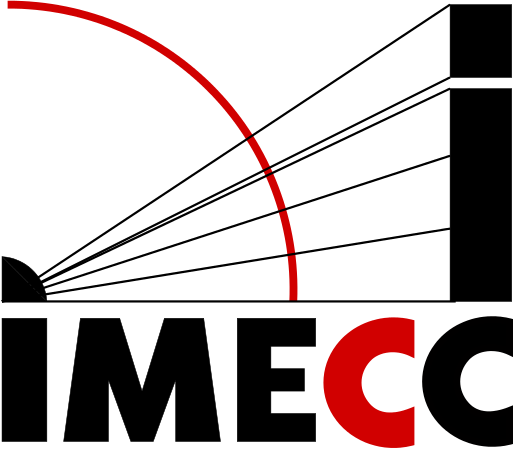
\includegraphics[width=0.2\textwidth]{logo-imecc (1) (1).png}\\ [0.1in]

{\large Universidade Estadual de Campinas}\\ [0.2cm] 
{\large Instituto de Matemática, Estatística e Matemática Computacional - IMECC}\\ [0.2cm] 
{\large Inferência Estatística na Era Computacional - ME904}\\ [5cm]


{\bf \Large Regressão Logística Penalizada}\\ [6cm]

{\large Bruno Martinez de Farias} \\ [0.2cm]
{\large Leonardo Mazzamboni Colussi} \\ [0.2cm]
{\large Vinícius Litvinoff Justus} \\ [2cm]  
 


{\large Campinas}\\ [0.2cm]
{\large 2021}

\end{center}
\end{titlepage}

\newpage
\pdfbookmark[0]{\contentsname}{toc}
\tableofcontents
\cleardoublepage

\section{Introdução}

\quad Um problema de regressão linear múltipla é um caso em que se
assume a estrutura
\(Y_i = \beta_0 + \sum_{j=1}^q \beta_j X_{ji} + \varepsilon_i\), onde
\(\varepsilon_i\), o termo de erro, é uma variável aleatória
\emph{i.i.d.} com distribuição normal, média \(\mu\) e variância
constante. Em outras palavras, assume-se que o valor esperado da
variável resposta \(Y_i\) é uma função linear das preditoras
\(X_{1i}, ..., X_{qi}\), com \(i = 1, ..., n\).

\quad No entanto, há muitas situações em que não é razoável assumir que
a variável resposta varie linearmente com relação às variáveis
independentes, podendo ser mais apropriado considerar uma função \(g\).
Esse tipo de problema motiva a criação dos modelos lineares
generalizados, onde \(Y_i|X_{1i}, ..., X_{qi}\) não é mais
necessariamente uma variável aleatória com distribuição normal. Mais
especificamente, na regressão logística, que é o caso particular de
modelo linear generalizado de interesse, assume-se que
\(Y_i|X_{1i}, ..., X_{qi}\) possui distribuição binomial.

\quad O objetivo deste trabalho é explorar a regressão logística
penalizada, ou seja, a aplicação de técnicas de regularização à
regressão logística. Para isto, a seção seguinte introduzirá a regressão
logística e os termos de penalização; na seção 3, será possível
visualizar o funcionamento do método através de simulações, e, por fim,
a última trará uma aplicação em dados reais.

\section{Metodologia}

\subsection{Regressão Logística}

\quad Embora seja possível aplicar a regressão logística em dados
multicategóricos, este trabalho focará na sua aplicação e interpretação
em dados binários. Assim, assume-se que se tem uma variável resposta
\(Y_i\) binária e se deseja estimar a probabilidade de \(Y_i = 1\) com
base nas variáveis explicativas \(X_{1i}, ...,X_{qi}\). Uma solução
ingênua para o problema é modelar uma regressão linear, da forma
\(E(Y_i|X_{1i},...,X_{qi}) = \beta_0 + \sum_{j=1}^q \beta_j X_{ji}\).

\quad Desse modo, a menos que todos os coeficientes (com exceção do
intercepto) sejam nulos - o que parece extremamente implausível -, a
esperança condicional de \(Y_i|X_{1i}, ..., X_{qi}\) será uma reta,
plano ou hiperplano, o que, inevitavelmente, acarreta na possibilidade
de se estimar probabilidades negativas ou maiores do que 1. Isto,
evidentemente, é problemático e implica no descarte da regressão linear
como modelo de um estudo cuja variável resposta é categórica.

\quad Uma possibilidade mais interessante é, ao invés de se modelar a
probabilidade \(p_i\), modelar a chance \(r_i\), representada na Equação
\ref{eq:chances}.

\begin{eqnarray}
\label{eq:chances}
r_i = \frac{p_i}{1 - p_i}.
\end{eqnarray}

\quad É possível demonstrar que existe uma relação \(1:1\) entre \(p_i\)
e \(r_i\), de modo que existe uma única chance associada a cada
probabilidade e vice-versa. Também é possível notar que, para
\(p_i \in (0,1)\), \(r_i \in (0, \infty)\).

\quad Então, a Equação \ref{eq:logit} expressa a função \emph{logit} (ou
log da chance), que modela linearmente a chance obtida da Equação
\ref{eq:chances}.

\begin{eqnarray}
\label{eq:logit}
g(p_i)= log \Big( \frac{p_i}{1 - p_i} \Big) = \beta_0 + \sum_{j=1}^q  \beta_j X_{ji}.
\end{eqnarray}

\quad Agora, finalmente, tem-se a função \(g\) de ligação do modelo
linear generalizado. Se o log da chance varia linearmente com relação às
preditoras, então as chances são funções de uma exponencial, o que
significa que, de fato, essas sempre serão positivas. Logo, veja que as
expressões obtidas das Equações \ref{eq:logit} e \ref{eq:logit2} são
equivalentes.

\begin{eqnarray}
\label{eq:logit2}
p_i = \frac{1}{1 + e^{-(\beta_0 + \sum_{j=1}^q  \beta_j X_{ji})}}.
\end{eqnarray}

\quad Assim, estimando as \emph{logit}'s, pode-se recuperar as
estimativas das probabilidades \(p_i\).

\subsection{\textit{Ridge} e \textit{Lasso}}

\quad Existe várias maneiras de se estimar os coeficientes \(\beta_j\)'s
de uma regressão logística. Usualmente, utiliza-se os estimadores de
mínimos quadrados ordinários, ou seja, busca-se os coeficientes que
minimizam a soma de quadrados dos resíduos, representada pela Equação
\ref{eq:difquad}.

\begin{eqnarray}
\label{eq:difquad}
\sum_{i=1}^{n}(\hat{y}_i - y_i)^2.
\end{eqnarray}

\quad Na regressão com regularização \(\ell_2\) (\emph{ridge}), a
expressão que se deseja minimizar (originalmente, a soma de quadrados
dos resíduos) recebe um novo termo que depende do tamanho dos
coeficientes \(\beta_{j, j \geq 1}\)'s. Assim, deseja-se minimizar a
Equação \ref{eq:reg}.

\begin{eqnarray}
\label{eq:reg}
\sum_{i=1}^{n}(\hat{y}_i - y_i)^2 + \lambda \sum_{j=1}^{q}(\beta_j)^2,
\end{eqnarray}

em que \(\lambda\) é um parâmetro de ajuste fino, atuando na seleção de
parâmetros \(\beta_{j, j \geq 1}\)'s mais influentes para o modelo. Na
prática, \(\lambda\) é determinado via validação cruzada ou via divisão
de dados em treinamento e validação, quando a base de dados utilizada é
consideravelmente grande.

\quad A regressão com regularização \(\ell_1\) (\emph{lasso}) opera de
maneira semelhante, mudando apenas o mecanismo de penalização, dada pela
Equação \ref{eq:lasso}.

\begin{eqnarray}
\label{eq:lasso}
\sum_{i=1}^{n}(\hat{y}_i - y_i)^2 + \lambda \sum_{j=1}^{q}|\beta_j|,
\end{eqnarray}

tal que \(\lambda\) não necessariamente é o mesmo parâmetro adotado na
\emph{ridge}.

\quad Há várias razões práticas pelo qual se pode adotar as técnicas de
regularização, dentre as quais se cita:

\begin{itemize}
\item A penalização do tamanho dos coeficientes evita o \textit{overfitting}, já que introduz um pequeno viés na estimativa através da introdução do coeficiente $\lambda$ na matriz que precisa ser invertida;
\item A eventual presença de multicolinearidade entre preditoras é corrigida;
\item Situações em que há mais preditoras do que observações, a introdução do termo de penalização também garante a unicidade da estimativa.
\end{itemize}

\section{Simulações}

\quad Para essa seção, realizou-se simulações com duas amostras de
tamanhos distintos, cada uma com 100 replicações, ambas com quatro
variáveis simuladas de forma diferente entre si e, para cada replicação,
foi armazenada uma semente com os estimadores dos parâmetros de uma
regressão logística não penalizada, penalizada pela regularização
\(\ell_1\) (\emph{lasso}) e, por último, pela regularização \(\ell_2\)
(\emph{ridge}). Assim, obteve-se a média das estimativas de cada
parâmetro, assim como o desvio padrão (DP) e o erro quadrático médio
(EQM). Ainda, simulou-se uma amostra da forma \(n < q\), em que \(n\) e
\(q\) são os números de observações da amostra e de parâmetros,
respectivamente.

\quad Sendo assim, as variáveis simuladas foram:

\begin{itemize}
\item $X_1$: variável binária, com probabilidade igual a $50\%$ de pertencer a uma das classes;
\item $X_2$: variável binária, no entanto, desbalanceada, com $90\%$ de pertencer à primeira classe e $10\%$ à segunda;
\item $X_3$: variável com 3 classes, distribuídas uniformemente;
\item $X_4$: variável numérica, gerada conforme uma distribuição uniforme no intervalo de 18 a 60, com valores inteiros.
\end{itemize}

\quad Inicialmente, simulou-se os dados de uma amostra de tamanho igual
a \(n = 100\) com \(100\) replicações, obtendo estimativas dos
parâmetros \footnote{Os valores verdadeiros dos parâmetros são:
  \(\beta_0=-9\), \(\beta_1=1\), \(\beta_2=3,7\), \(\beta_3=0,4\),
  \(\beta_4=0,5\), \(\beta_5=0,2\).} para cada método, conforme a Tabela
\ref{tab:tabsim1}.

\begin{table}[H]

\caption{\label{tab:tabsim1}Simulação de amostras de tamanho 100, com 100 replicações.}
\centering
\fontsize{10}{12}\selectfont
\begin{tabular}[t]{lrrrrrrrrr}
\toprule
\multicolumn{1}{c}{ } & \multicolumn{3}{c}{Sem penalização} & \multicolumn{3}{c}{Penalização Ridge} & \multicolumn{3}{c}{Penalização Lasso} \\
\cmidrule(l{3pt}r{3pt}){2-4} \cmidrule(l{3pt}r{3pt}){5-7} \cmidrule(l{3pt}r{3pt}){8-10}
  & Média & DP & EQM & Média & DP & EQM & Média & DP & EQM\\
\midrule
$\hat{\beta}_0$ & -10,517 & 2,498 & 8,542 & -5,816 & 0,633 & 10,540 & -7,620 & 1,790 & 5,109\\
$\hat{\beta}_1$ & 1,256 & 0,787 & 0,684 & 0,611 & 0,375 & 0,292 & 0,666 & 0,573 & 0,440\\
$\hat{\beta}_2$ & 6,622 & 6,235 & 47,414 & 2,130 & 0,775 & 3,065 & 2,675 & 1,499 & 3,298\\
$\hat{\beta}_3$ & 0,340 & 0,863 & 0,748 & 0,086 & 0,451 & 0,302 & 0,133 & 0,532 & 0,354\\
$\hat{\beta}_4$ & 0,587 & 0,911 & 0,838 & 0,264 & 0,499 & 0,305 & 0,266 & 0,575 & 0,386\\
$\hat{\beta}_5$ & 0,235 & 0,055 & 0,004 & 0,133 & 0,014 & 0,005 & 0,177 & 0,040 & 0,002\\
\bottomrule
\end{tabular}
\end{table}

\quad Dessa forma, nota-se que, para esse primeiro caso, as estimativas
com menor EQM são obtidas pelo método da regressão logística com
regularização \(\ell_1\), enquanto para a regularização \(\ell_2\) o
viés é consideravelmente alto, o que implica no alto EQM. No que tange
às estimativas referentes à regressão logística sem penalidade, os
estimadores são obtidos pelo método de máxima verossimilhança, cujos
parâmetros têm boas propriedades assintóticas. Logo, conforme o tamanho
da amostra aumenta, as estimativas tendem a ser melhores para seus
respectivos parâmetros.

\quad Aumentando o tamanho da amostra para \(n = 1000\), obteve-se as
estimativas da Tabela \ref{tab:tabsim2}. Como dito anteriormente, é
esperado que as estimativas para a regressão logística sem penalidade
sejam mais próximas aos verdadeiros valores dos parâmetros, conforme
\(n \rightarrow \infty\). No entanto, os valores das estimativas para a
regularização \(\ell_1\) se apresentaram bem próximos aos valores reais
dos parâmetros, mesmo que o método tenha como objetivo inserir um
pequeno viés aos estimadores, com a intenção de diminuir a variância
destes. Por sua vez, a regularização \(\ell_2\) apresentou os piores
valores estimados para cada parâmetro.

\begin{table}[H]

\caption{\label{tab:tabsim2}Simulação de amostras de tamanho 1000, com 100 replicações.}
\centering
\fontsize{10}{12}\selectfont
\begin{tabular}[t]{lrrlrrrrrl}
\toprule
\multicolumn{1}{c}{ } & \multicolumn{3}{c}{Sem penalização} & \multicolumn{3}{c}{Penalização Ridge} & \multicolumn{3}{c}{Penalização Lasso} \\
\cmidrule(l{3pt}r{3pt}){2-4} \cmidrule(l{3pt}r{3pt}){5-7} \cmidrule(l{3pt}r{3pt}){8-10}
  & Média & DP & EQM & Média & DP & EQM & Média & DP & EQM\\
\midrule
$\hat{\beta}_0$ & -9,109 & 0,580 & 0,348 & -5,742 & 0,222 & 10,662 & -8,816 & 0,720 & 0,552\\
$\hat{\beta}_1$ & 1,018 & 0,202 & 0,041 & 0,591 & 0,115 & 0,181 & 0,954 & 0,211 & 0,047\\
$\hat{\beta}_2$ & 3,759 & 0,403 & 0,166 & 2,177 & 0,195 & 2,357 & 3,612 & 0,411 & 0,177\\
$\hat{\beta}_3$ & 0,411 & 0,231 & 0,053 & 0,185 & 0,147 & 0,068 & 0,321 & 0,265 & 0,076\\
$\hat{\beta}_4$ & 0,496 & 0,232 & 0,054 & 0,256 & 0,156 & 0,084 & 0,434 & 0,295 & 0,091\\
$\hat{\beta}_5$ & 0,202 & 0,012 & <0,001 & 0,130 & 0,004 & 0,005 & 0,197 & 0,013 & <0,001\\
\bottomrule
\end{tabular}
\end{table}

\quad Assim, extraiu-se uma das amostras da simulação e construiu-se o
gráfico da Figura \ref{fig:coefs}. Desse modo, é possível notar que os
coeficientes relacionados às variáveis menos influentes para o modelo
zeram mais rapidamente para o caso da regularização \(\ell_1\) quando
comparado à regularização \(\ell_2\). Ainda, o valores obtidos de
\(\lambda\) para esta primeira é consideravelmente menor do que para a
segunda regularização, o que é condizente com a interpretação realizada.

\begin{figure}

{\centering \includegraphics{trabalho01_ME904_files/figure-latex/coefs-1} 

}

\caption{Gráficos dos valores de lambda em relação aos coeficientes obtidos da regularização Lasso e Ridge.}\label{fig:coefs}
\end{figure}

\newpage

\quad Para finalizar a seção, simulou-se um caso \(n<q\), \(n = 1000\) e
\(q = 2000\), de forma que os valores de cada variável preditora foram
gerados com base em uma distribuição normal padrão. Além disso, dado o
grande número de parâmetros, a simulação foi feita de forma que apenas
os três primeiros fossem significativos, conforme a Equação
\ref{eq:betas}.

\begin{eqnarray}
\label{eq:betas}
\begin{cases}
\beta_j = 1, \text{ para } j = 1, 2 \text{ e } 3; \\
\beta_j = 0, \text{ para } 3 < j \leq 2000.
\end{cases}
\end{eqnarray}

\quad Da Figura \ref{fig:coefs2}, nota-se que os coeficientes simulados
como zero convergiram rapidamente para esse valor, no caso da
regularização \(\ell_1\). Em contrapartida, utilizando-se a
regularização \(\ell_2\), os valores dos coeficientes nunca convergem
para o valor nulo, por mais próximo que seja, \(\forall \lambda\). Além
disso, para esse segundo método, a desprezível influência dos
coeficientes simulados com valores nulos não foi percebida de imediato,
dado o grande intervalo de valores considerado para o parâmetro de
afinação, quando comparado ao primeiro método.

\begin{figure}

{\centering \includegraphics{trabalho01_ME904_files/figure-latex/coefs2-1} 

}

\caption{Gráficos dos valores de lambda em relação aos coeficientes obtidos da regularização Lasso e Ridge, para n < p.}\label{fig:coefs2}
\end{figure}

\section{Aplicação dos Métodos}

\quad Para os ajustes dos modelos de regressão logística com
regularização \(\ell_1\) e \(\ell_2\), o banco de dados utilizado foi
particionado aleatóriamente em três conjuntos distintos. O primeiro,
base de treinamento, contém \(60\%\) da amostra, em que os modelos são
ajustados com o objetivo de encontrar o parâmetro de afinação
\(\lambda\), por meio de validação cruzada. O segundo, dados de
validação, que representam \(20\%\) da amostra, são aplicados aos
ajustes feitos, de modo que a indicação do melhor modelo é realizada com
base no EQM dos dados de validação. Sendo assim, após a escolha do
melhor modelo e seu respectivo parâmetro de afinação, ajusta-se um novo
modelo, agora com os dados de treino e validação conjuntamente. Por fim,
o melhor modelo proposto é aplicado aos dados de teste, que compõem os
\(20\%\) restantes da amostra, para analisar se este apresenta boa
performance para dados não utilizados em treinamento e validação.

\newpage

\subsection{Análise Descritiva}

\quad O conjunto de dados utilizado nessa seção se referem a um estudo
feito por médicos residentes na cidade de Framingham, Massachussets,
sobre doenças cardíacas. Desse modo, o problema de classificação tem
como propósito prever se um paciente tem risco de desenvolver doença
cardíaca coronária nos próximos dez anos, com base em algumas
informações sobre eles, apresentadas na Tabela \ref{tab:vars}. O banco
de dados pode ser encontrado em
\href{https://www.kaggle.com/naveengowda16/logistic-regression-heart-disease-prediction}{\textit{Heart Disease Prediction}}.

\quad O banco é composto por quinze variáveis, oito delas são contínuas
e sete são categóricas, em que \texttt{Risco10anos} é a variável
resposta binária (desbalanceada), indicando se o paciente apresenta
risco de desenvolver doença cardíaca nos próximos 10 anos. Na Figura 3
está indicada a correlação entre as variáveis do banco de dados, onde
pode ser observado que as variáveis \texttt{PSSist} e \texttt{PSDias}
apresentam alta correlação (0,794), assim como \texttt{PSMeds} e
\texttt{Hipertensão} (\(0,970\)), \texttt{PSSist} e \texttt{Hipertensão}
(\(0,848\)), \texttt{PSDias} e \texttt{Hipertensão} (\(0,774\)) e, por
fim, \texttt{Fumante} e \texttt{CigsPorDia} (\(0,903\)), certamente.

\quad Em relação à variável \texttt{PSSist}, que se refere à pressão
arterial sistólica, observa-se um nível mais elevado em pacientes com
risco de doença cardíaca, conforme a Figura \ref{fig:pssist}.
Entretanto, as demais variáveis contínuas apresentam distribuições
similares em relação aos grupos de pacientes com base na variável
resposta.

\quad Ainda, na Figura \ref{fig:age}, é possível observar a distribuição
das idades dos pacientes agrupados por ausência ou presença do risco de
doença cardíaca. Apesar do número inferior de pacientes com risco, é
possível notar que, quanto maior a idade, maior é o número de pacientes
com doenças cardíacas e, em contrapartida, o número de pacientes sem
risco diminui.

\quad Na Tabela \ref{tab:sex}, tem-se a distribuição dos sexos dos
pacientes. Assim, independentemente do risco, nota-se a predominância do
sexo feminino entre os pacientes. Além disso, a doença cardíaca se
mostra mais presente para pacientes com casos de hipertensão, conforme a
distribuição da variável \texttt{Hipertensão}. No entanto, as demais
variáveis categóricas apresentam maior frequência para a classe \(0\).

\subsection{Modelagem}

\quad Nesta seção será realizado o ajuste dos modelos de regressão
logística utilizando as regularizações \(\ell_1\) (\emph{lasso}) e
\(\ell_2\) (\emph{ridge}) para o conjunto de treinamento. Sendo assim,
obteve-se o valor de \(\lambda_{lasso}=\) 0,00545 e
\(\lambda_{ridge} =\) 0,0141, para os parâmetros de afinação da
regressão logística com as regularizações \emph{lasso} e \emph{ridge},
respectivamente, por meio do método de validação cruzada.

\quad Apenas com os parâmetros \(\beta_j\)'s estimados, é possível
observar como a regularização influencia consideravelmente na seleção de
variáveis no modelo. Na Tabela \ref{tab:coefi_final}, nota-se que, por
um lado, a regularização aplicada pelo parâmetro de afinação
\(\lambda_{ridge}\) não anula nenhum dos \(\beta_{j, j \geq 1}\)'s, por
menor que sejam. Por outro, a regularização \emph{lasso} apresentou sete
parâmetros significantes para o modelo, zerando os demais. Dessa forma,
a Tabela \ref{tab:coefi_final} apresenta os coeficientes ajustados no
modelo de treinamento.

\quad Das duas penalizações utilizadas para o ajuste, o modelo com
penalização \(\ell_1\) apresentou o menor erro quadrático médio (EQM),
tanto em relação aos dados de treinamento, quanto aos dados de validação
e, consequentemente, possui a menor taxa de erro de predição. Na Tabela
\ref{tab:aval} estão presentes os EQM's dos dois modelos ajustados nos
conjuntos de treinamento e validação.

\begin{table}[H]

\caption{\label{tab:aval}Tabela de EQM por método de ajuste de modelo.}
\centering
\fontsize{10}{12}\selectfont
\begin{tabular}[t]{lrr}
\toprule
Modelo & EQM de Treino & EQM de Validação\\
\midrule
Ridge & 5,064 & 5,001\\
Lasso & 4,965 & 4,896\\
\bottomrule
\end{tabular}
\end{table}

\quad Sendo assim, o modelo com regularização \(\ell_1\), cujo parâmetro
de afinação é \(\lambda_{lasso}=\) 0,0055, foi escolhido como ajuste
final. Posteriormente a esse passo, reajustou-se novamente o modelo, no
entanto, agora considerando os dados de treinamento e validação
conjuntamente, mantendo o parâmetro de afinação obtido, o que resultou
nos coeficientes da Tabela \ref{tab:coefi_final}.

\quad Portanto, o modelo final com as variáveis mais influentes para
esse estudo é dado pela Equação \ref{eq:modelofinal}.

\begin{eqnarray}
\label{eq:modelofinal}
\log\left(\dfrac{p_i}{1-p_i}\right) &=& -6,393 + 0,376 \cdot \text{Sexo} + 0,051\cdot \text{Idade} + 0,01 \cdot \text{CigsPorDia}\nonumber \\
+ 0,013 \cdot \text{AVC} &+& 0,184 \cdot \text{Hipertensão} + 0,01 \cdot \text{PSSist} + 0,004 \cdot \text{Glicose}.
\end{eqnarray}

\subsection{Diagnóstico do Modelo}

\quad O modelo de regressão logística associa uma probabilidade \(p_i\)
de \(Y_i = 1\) a cada conjunto \(X_{1i},...,X_{qi}\) de preditoras.
Contudo, o objetivo final do modelo é, através dessas variáveis
preditoras, obter uma regra que associe uma categoria para \(Y_i\) aos
dados utilizados. Deste modo, faz-se necessário estabelecer um ponto de
corte, isto é, fixar uma quantidade \(p_i^* \in (0,1)\) tal que, a cada
valor \(p_i\), associa-se o valor \(1\) à variável \(Y_i\) se
\(p_i > p_i^*\) e \(0\) caso contrário.

\quad A Tabela \ref{tab:mat} apresenta a matriz de confusão do modelo
com regularização \emph{lasso} para algumas possíveis probabilidades de
corte, \(p_i\), que determina a associação da variável resposta ao nível
\(1\). No contexto do banco de dados escolhido, essa é a probabilidade
que associa um paciente a ser classificado como pessoa que apresenta
risco de desenvolver doença cardíaca nos próximos dez anos.

\begin{table}[H]

\caption{\label{tab:mat}Matriz de confusão para as probabilidades de corte iguais a 0,1;  0,2;  0,3;  0,4 e  0,5.}
\centering
\fontsize{9}{11}\selectfont
\begin{tabular}[t]{lrrrrrrrrrr}
\toprule
\multicolumn{1}{c}{ } & \multicolumn{10}{c}{Predição} \\
\cmidrule(l{3pt}r{3pt}){2-11}
\multicolumn{1}{c}{ } & \multicolumn{2}{c}{Prob. de Corte 0,1} & \multicolumn{2}{c}{Prob. de Corte 0,2} & \multicolumn{2}{c}{Prob. de Corte 0,3} & \multicolumn{2}{c}{Prob. de Corte 0,4} & \multicolumn{2}{c}{Prob. de Corte 0,5} \\
\cmidrule(l{3pt}r{3pt}){2-3} \cmidrule(l{3pt}r{3pt}){4-5} \cmidrule(l{3pt}r{3pt}){6-7} \cmidrule(l{3pt}r{3pt}){8-9} \cmidrule(l{3pt}r{3pt}){10-11}
Referência & 0 & 1 & 0 & 1 & 0 & 1 & 0 & 1 & 0 & 1\\
\midrule
0 & 289 & 347 & 509 & 127 & 601 & 35 & 629 & 7 & 635 & 1\\
1 & 16 & 99 & 51 & 64 & 90 & 25 & 101 & 14 & 111 & 4\\
\bottomrule
\end{tabular}
\end{table}

\quad Analisando as possíveis probabilidades de corte, quando
\(p_i^* = 0,10\), tem-se que a proporção de verdadeiros-positivos é de
0,86 e 0,55 para falsos-positivos. No caso em que \(p_i^* = 0,20\), a
proporção do primeiro reduz para 0,56 e a proporção do segundo decai
para 0,2. A partir de um ponto de corte \(p_i^*=0,30\), a proporção de
verdadeiros-positivos é inferior a 0,22, o que dificulta a identificação
de pacientes com um real risco de doenças cardíacas. Sendo assim, a
disposição dos pontos de corte em relação às taxas de
verdadeiros-positivos e falsos-positivos podem ser observadas na Figura
\(10\), que apresenta o gráfico da curva \emph{ROC} do modelo ajustado.

\quad Apesar da acurácia balanceada ser de \(82,56\%\) para uma
probabilidade de corte \(p_i^* = 0,5\), com base no gráfico da Figura
\(10\) e no contexto do banco de dados utilizado, um falso-positivo, por
mais inapropriado que seja, é conivente com o objetivo do estudo na
prevenção de doenças cardíacas em relação a um falso-negativo. Por esse
motivo, um ponto de corte aceitável para o problema de classificação
seria \(p_i^* = 0,15\), com aproximadamente \(60\%\) de acurácia
balanceada.

\subsection{Interpretação do Modelo}

\quad Para a interpretação do modelo, foi considerado um paciente do
sexo masculino, com \(50\) anos de idade, não fumante, que faz uso de
medicamentos para controle de pressão arterial, já teve um AVC e tem
histórico de hipertensão, mas não de diabetes. Dessa forma, mediu-se a
pressão sistólica e o nível de glicose do paciente, obtendo um valor de
\(132,4\) \(mmHg\) e \(71\) \(mg/dl\), respectivamente.

\quad Assim, o modelo ajustado prediz, para esse paciente, a
probabilidade obtida na Equação \ref{eq:result}.

\begin{eqnarray}
\log\left(\dfrac{p_i}{1-p_i}\right) &=& -6,393 + 0,376 \cdot 1 + 0,051\cdot 50 + 0,01 \cdot 0\nonumber\\
&+& 0,013 1 + 0,184 \cdot 1 + 0,01 \cdot 132,4 + 0,004 \cdot 71.
\end{eqnarray}

Logo,

\begin{eqnarray}
\label{eq:result}
\log\left(\dfrac{p_i}{1-p_i}\right) &=& -2,216; \nonumber \\
p_i &=& \dfrac{1}{1+e^{-(-2,216)}}; \nonumber \\
p_i &=& 0,1616.
\end{eqnarray}

\quad Sob tais condições, a probabilidade desse paciente desenvolver
doença cardíaca é de, aproximadamente, \(16,16\%\), superior à
probabilidade de corte \(p_i^*=0,15\) estabelecida. Dessa maneira, ele
seria classificado como paciente que apresenta risco de desenvolver uma
doença cardíaca nos próximos dez anos.

\newpage

\begin{thebibliography}{9}
\bibitem{link(1)}\url{https://www.who.int/en/news-room/fact-sheets/detail/cardiovascular-diseases-(cvds)}\\
\bibitem{link(1)}\text{JAMES, Gareth et al. An introduction to statistical learning, Springer, Nova Iorque, 2013.}\\
\bibitem{link(1)}\text{FRANKLIN, James. The elements of statistical learning: data mining, inference and prediction.} \\
\text{The Mathematical Intelligencer, v. 27, n. 2, p. 83-85, 2005.}
\end{thebibliography}

\newpage
\section{Apêndices}

\subsection{Tabelas}

\begin{table}[H]

\caption{\label{tab:vars}Descrição das variáveis presentes no banco de dados.}
\centering
\fontsize{10}{12}\selectfont
\begin{tabular}[t]{ll}
\toprule
Variáveis & Descrição\\
\midrule
Sexo & Sexo Masculino ou Feminino (Categórica)\\
Idade & Idade do paciênte (Contínua)\\
Fumante & Se o paciente é ou não fumante (Categórica)\\
CigsPorDia & Número de cigarros por dia (Contínua)\\
PSMeds & Se o paciente faz uso de medicamento para controle de pressão arterial (Categórica)\\
AVC & Se o paciente já sofreu um acidente vascular cerebral (Categórica)\\
Hipertensão & Se o paciente é hipertenso ou não (Categórica)\\
Diabetes & Se o paciente tem ou não diabetes (Categórica)\\
ColTotal & Nível de colesterol total (Contínua)\\
PSSist & Pressão sanguinêa sistólica (Contínua)\\
PSDias & Pressão sanguinêa diastólica (Contínua)\\
IMC & Índice de massa corporal (Contínua)\\
FreqCard & Frequência cardíaca (Contínua)\\
Glicose & Nível de glicose (Contínua)\\
Risco10anos & Risco de doença cardíaca coronária em 10 anos (Categórica)\\
\bottomrule
\end{tabular}
\end{table}

\begin{table}[H]
\caption{\label{tab:sex}Tabela de contingência das variáveis Sexo e Fumante.}

\centering
\fontsize{10}{12}\selectfont
\begin{tabular}[t]{lll}
\toprule
Risco & Masculino & Feminino\\
\midrule
Sem Risco & 0,358 & 0,490\\
Com risco & 0,086 & 0,066\\
\bottomrule
\end{tabular}
\centering
\begin{tabular}[t]{lll}
\toprule
Risco & Nao\_fumante & Fumante\\
\midrule
Sem Risco & 0,442 & 0,405\\
Com risco & 0,073 & 0,079\\
\bottomrule
\end{tabular}
\end{table}

\begin{table}[H]
\caption{\label{tab:meds}Tabela de contingência das variáveis PSMeds e AVC.}

\centering
\fontsize{10}{12}\selectfont
\begin{tabular}[t]{lll}
\toprule
Risco & Nao\_usa & Usa\\
\midrule
Sem Risco & 0,82 & 0,0230\\
Com risco & 0,14 & 0,0087\\
\bottomrule
\end{tabular}
\centering
\begin{tabular}[t]{lll}
\toprule
Risco & Nao\_teve & Teve\\
\midrule
Sem Risco & 0,84 & 0,0033\\
Com risco & 0,15 & 0,0023\\
\bottomrule
\end{tabular}
\end{table}

\begin{table}[H]
\caption{\label{tab:hiper}Tabela de contingência das variáveis Hipertensão e Diabetes.}

\centering
\fontsize{10}{12}\selectfont
\begin{tabular}[t]{lll}
\toprule
Risco & Nao\_hiper & hipertenso\\
\midrule
Sem Risco & 0,610 & 0,237\\
Com risco & 0,074 & 0,078\\
\bottomrule
\end{tabular}
\centering
\begin{tabular}[t]{lll}
\toprule
Risco & Nao\_diab & diabetes\\
\midrule
Sem Risco & 0,83 & 0,0187\\
Com risco & 0,14 & 0,0097\\
\bottomrule
\end{tabular}
\end{table}

\begin{table}[H]

\caption{\label{tab:coefi_final}Coeficientes do modelo com regularização ridge (Treino), lasso (Treino) e lasso (Treino e Validação).}
\centering
\fontsize{10}{12}\selectfont
\begin{tabular}[t]{lrrr}
\toprule
  & Estimadores Ridge (Treino) & Estimadores Lasso (Treino) & Estimadores Lasso (Treino com Validação)\\
\midrule
$\hat{\beta}_0$ & -7,530 & -7,572 & -6,393\\
$\hat{\beta}_1$ & 0,544 & 0,525 & 0,376\\
$\hat{\beta}_2$ & 0,057 & 0,060 & 0,051\\
$\hat{\beta}_3$ & 0,120 & 0,000 & 0,000\\
$\hat{\beta}_4$ & 0,018 & 0,019 & 0,010\\
$\hat{\beta}_5$ & -0,350 & -0,107 & 0,000\\
$\hat{\beta}_6$ & 1,350 & 1,020 & 0,013\\
$\hat{\beta}_7$ & 0,288 & 0,177 & 0,184\\
$\hat{\beta}_8$ & 0,106 & 0,000 & 0,000\\
$\hat{\beta}_9$ & 0,001 & 0,000 & 0,000\\
$\hat{\beta}_{10}$ & 0,014 & 0,013 & 0,010\\
$\hat{\beta}_{11}$ & -0,005 & 0,000 & 0,000\\
$\hat{\beta}_{12}$ & 0,018 & 0,006 & 0,000\\
$\hat{\beta}_{13}$ & -0,004 & 0,000 & 0,000\\
$\hat{\beta}_{14}$ & 0,004 & 0,004 & 0,004\\
\bottomrule
\end{tabular}
\end{table}

\newpage

\subsection{Gráficos}

\begin{figure}
\centering
\includegraphics{trabalho01_ME904_files/figure-latex/cor-1.pdf}
\caption{Correlação entre as variáveis preditoras.}
\end{figure}

\begin{figure}

{\centering \includegraphics{trabalho01_ME904_files/figure-latex/cigs-1} 

}

\caption{Boxplot do número de cigarros por dia  pelo risco de ter doença cardíaca em 10 anos.}\label{fig:cigs}
\end{figure}

\begin{figure}

{\centering \includegraphics{trabalho01_ME904_files/figure-latex/pssist-1} 

}

\caption{Boxplot da pressão sanguínea sistólica e diastólica por risco de ter doença cardíaca em 10 anos.}\label{fig:pssist}
\end{figure}

\begin{figure}

{\centering \includegraphics{trabalho01_ME904_files/figure-latex/IMC-1} 

}

\caption{Boxplots do nível de colesterol e IMC por risco de ter doença cardíaca em 10 anos.}\label{fig:IMC}
\end{figure}

\begin{figure}

{\centering \includegraphics{trabalho01_ME904_files/figure-latex/age-1} 

}

\caption{Histograma da idade conforme o risco de ter doença cardíaca em 10 anos.}\label{fig:age}
\end{figure}

\begin{figure}

{\centering \includegraphics{trabalho01_ME904_files/figure-latex/freq_cardio-1} 

}

\caption{Histograma da frequência cardíaca conforme o risco de ter doença cardíaca em 10 anos.}\label{fig:freq_cardio}
\end{figure}

\begin{figure}

{\centering \includegraphics{trabalho01_ME904_files/figure-latex/glico-1} 

}

\caption{Gráfico da densidade de probabilidade do nível de glicose.}\label{fig:glico}
\end{figure}

\begin{figure}
\centering
\includegraphics{trabalho01_ME904_files/figure-latex/Croc-1.pdf}
\caption{Curva ROC.}
\end{figure}

\end{document}
